% A schematic diagram showing the shape of the feature map as it passes through the network.

% In the encoding path, the feature map is transformed with two successive 3x3x3 convolutions and ReLU activations
% followed by a 2x2x2 max-pooling operation that reduces the spatial dimensions by half.

% In the decoding path, information from fine and coarse scales is combined through skip connections.
% The feature map is upsampled by a factor of 2 using a 3x3x3 transposed convolution.
% This is combined with the feature map from the contracting path through a skip connection,
% which is passed through an attention gate before being concatenated with the upsampled feature map.
% The feature map from deeper in the network acts as the attention gating signal.
% The upsampled feature map and attended feature map from the skip connection are concatenated and
% convolved along the channel dimension to produce the final feature map.

\documentclass{standalone}
\usepackage{tikz}
\usetikzlibrary{shapes.geometric, arrows.meta, positioning, calc}

% Styles
\tikzstyle{block} = [rectangle, draw, text centered, minimum width=2cm, minimum height=1cm, fill=white]
\tikzstyle{conv} = [thick, ->, >=stealth, black]
\tikzstyle{pool} = [thick, ->, >=stealth, blue]
\tikzstyle{up}   = [thick, ->, >=stealth, red]
\tikzstyle{skip} = [thick, dashed, ->, >=stealth, gray]
\tikzstyle{gate} = [thick, ->, >=stealth, violet]
\tikzstyle{attention} = [circle, draw, text centered, minimum size=1cm, fill=orange!20]
\tikzstyle{concat} = [draw, dotted, minimum width=1cm, minimum height=1cm]


\begin{document}
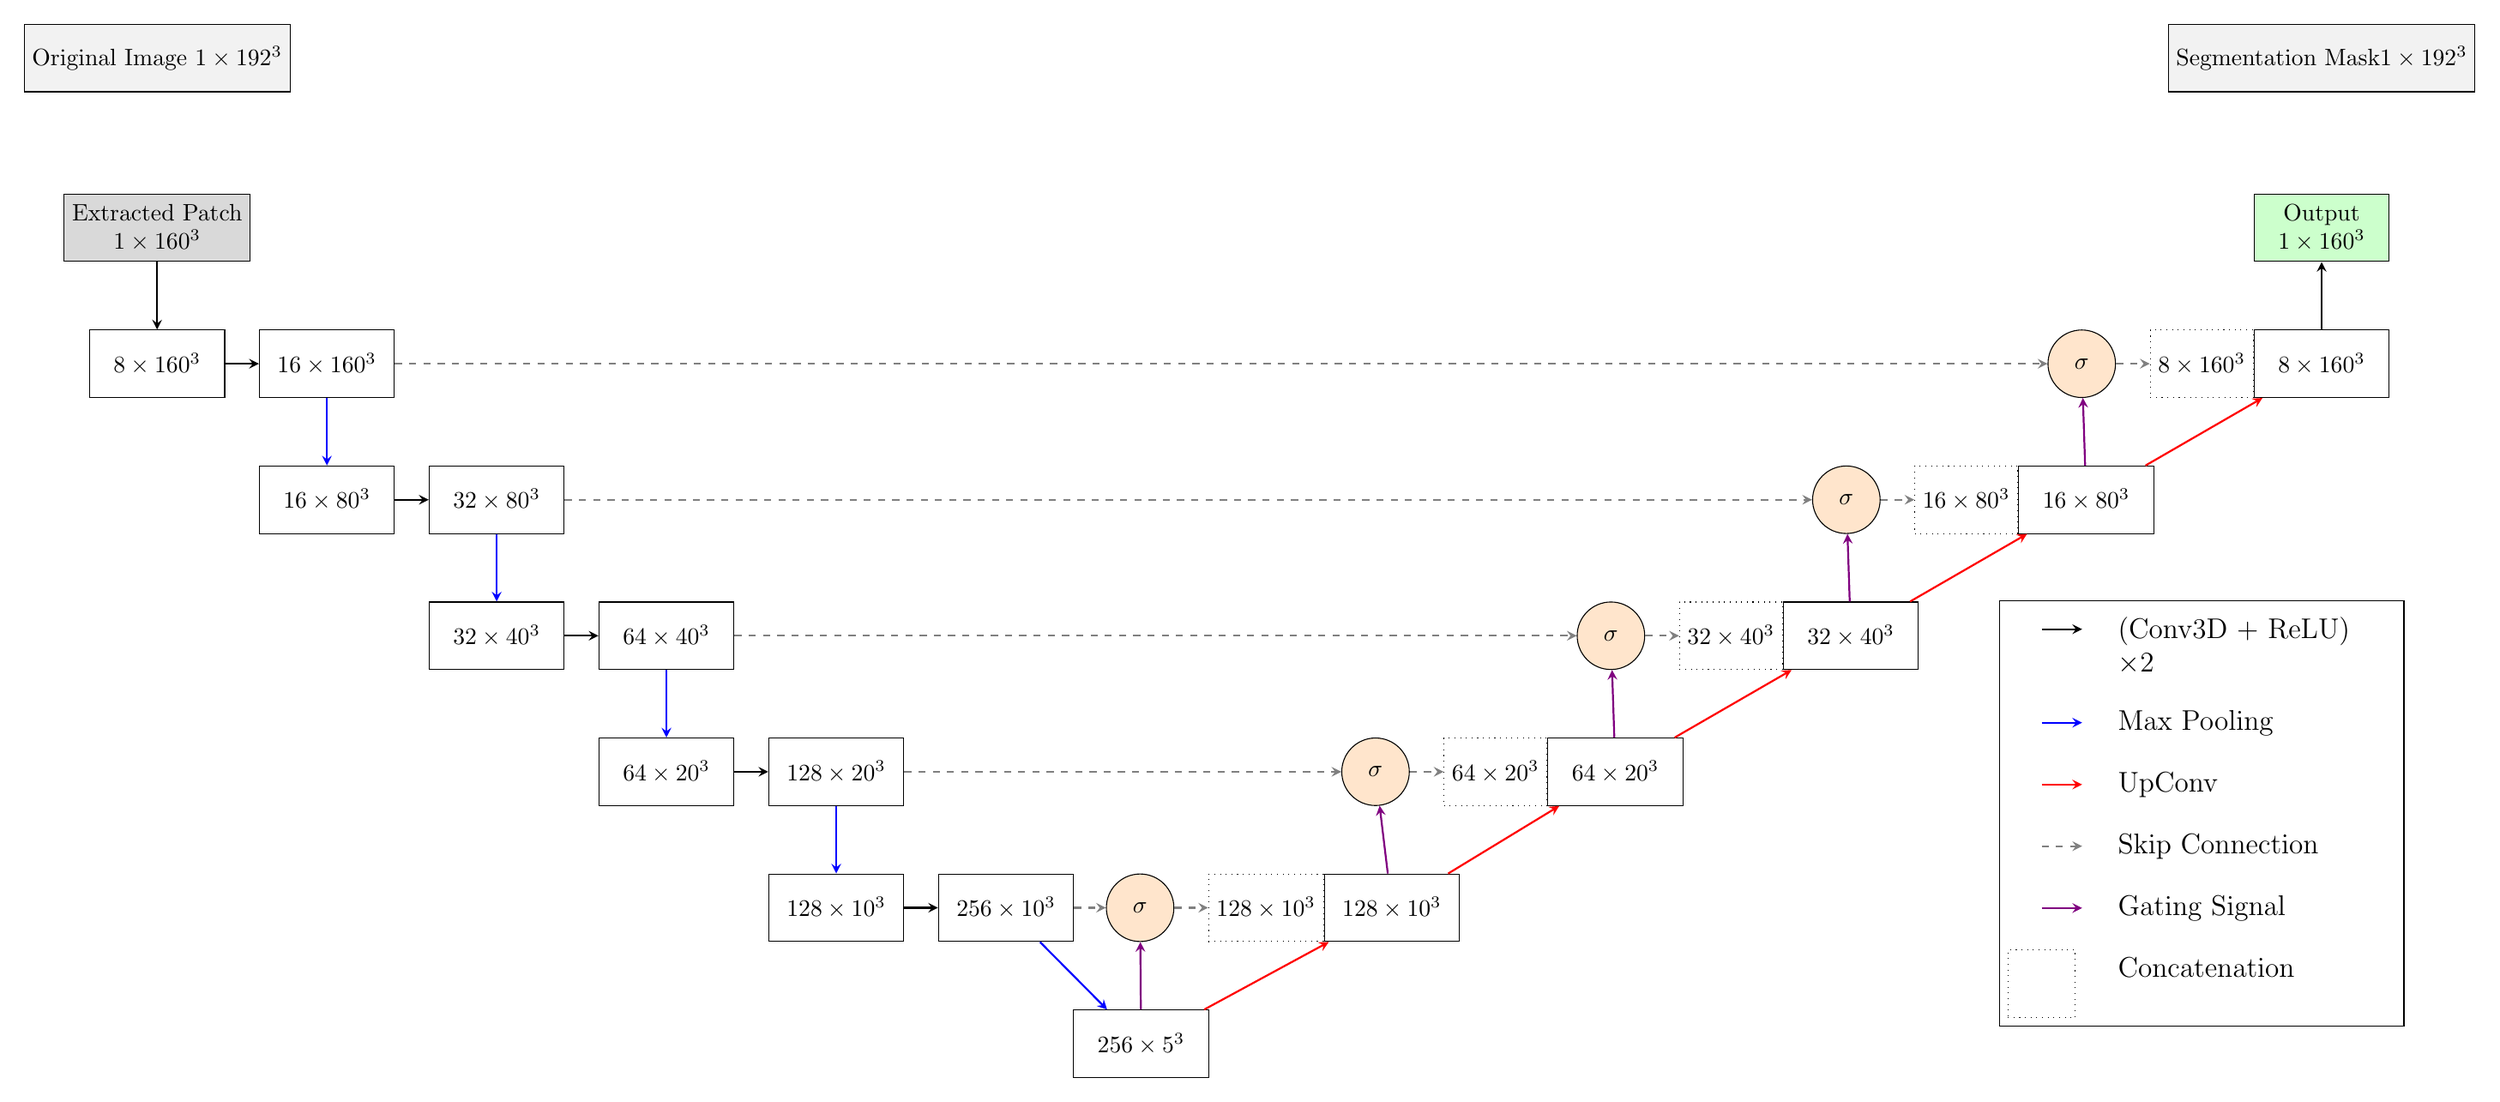
\begin{tikzpicture}[node distance=1.8cm and 0.5cm]

	% Input image and patch
	\node (input_full) [block, fill=gray!10] {Original Image $1\times192^3$};
	\node (input_patch) [block, below=1.5cm of input_full, fill=gray!30, align=center] {Extracted Patch\\$1\times160^3$};

	% Encoder
	\node (enc0) [block, below=1cm of input_patch] {$8\times160^3$};
	\node (enc1) [block, below right=1cm and 0.5cm of enc0] {$16\times80^3$};
	\node (enc2) [block, below right=1cm and 0.5cm of enc1] {$32\times40^3$};
	\node (enc3) [block, below right=1cm and 0.5cm of enc2] {$64\times20^3$};
	\node (enc4) [block, below right=1cm and 0.5cm of enc3] {$128\times10^3$};

	% Encoder - convolutions
	\node (enc0b) [block, right=0.5cm of enc0] {$16\times160^3$};
	\node (enc1b) [block, right=0.5cm of enc1] {$32\times80^3$};
	\node (enc2b) [block, right=0.5cm of enc2] {$64\times40^3$};
	\node (enc3b) [block, right=0.5cm of enc3] {$128\times20^3$};
	\node (enc4b) [block, right=0.5cm of enc4] {$256\times10^3$};

	% Decoder - skips
	\node (dec0) [concat, right=28.5cm of enc0] {$8\times160^3$};
	\node (dec1) [concat, right=22.5cm of enc1]   {$16\times80^3$};
	\node (dec2) [concat, right=16.5cm of  enc2]   {$32\times40^3$};
	\node (dec3) [concat, right=10.5cm of  enc3]   {$64\times20^3$};
	\node (dec4) [concat, right=4.5cm of  enc4]   {$128\times10^3$};

	% Decoder - upsampling
	\node (dec0b) [block, right=0cm of dec0] {$8\times160^3$};
	\node (dec1b) [block, right=0cm of dec1]   {$16\times80^3$};
	\node (dec2b) [block, right=0cm of dec2]   {$32\times40^3$};
	\node (dec3b) [block, right=0cm of dec3]   {$64\times20^3$};
	\node (dec4b) [block, right=0cm of dec4]   {$128\times10^3$};

	% Bottleneck
	\node (bottom) [block, below right=1cm and 2.5cm of enc4] {$256\times5^3$};

	% Attention Gates
	\node (att4) [attention, left=0.5cm of dec4] {$\sigma$};
	\node (att3) [attention, left=0.5cm of dec3] {$\sigma$};
	\node (att2) [attention, left=0.5cm of dec2] {$\sigma$};
	\node (att1) [attention, left=0.5cm of dec1] {$\sigma$};
	\node (att0) [attention, left=0.5cm of dec0] {$\sigma$};

	\node (output_patch) [block, above=1cm of dec0b, fill=green!20, align=center] {Output\\$1\times160^3$};
	\node (output_full) [block, fill=gray!10, above=1.5cm of output_patch] {Segmentation Mask$1\times192^3$};

	% Arrows - conv
	\draw[conv] (enc0) -- (enc0b);
	\draw[conv] (enc1) -- (enc1b);
	\draw[conv] (enc2) -- (enc2b);
	\draw[conv] (enc3) -- (enc3b);
	\draw[conv] (enc4) -- (enc4b);

	% Arrows - Encoder
	\draw[conv] (input_patch) -- (enc0);
	\draw[pool] (enc0b) -- (enc1);
	\draw[pool] (enc1b) -- (enc2);
	\draw[pool] (enc2b) -- (enc3);
	\draw[pool] (enc3b) -- (enc4);
	\draw[pool] (enc4b) -- (bottom);

	% Arrows - Decoder
	\draw[up] (bottom) -- (dec4b);
	\draw[up] (dec4b) -- (dec3b);
	\draw[up] (dec3b) -- (dec2b);
	\draw[up] (dec2b) -- (dec1b);
	\draw[up] (dec1b) -- (dec0b);
	\draw[conv] (dec0b) -- (output_patch);

	% Skip Connections with Attention
	\draw[skip] (enc4b) -- (att4);
	\draw[skip] (att4) -- (dec4);
	\draw[skip] (enc3b) -- (att3);
	\draw[skip] (att3) -- (dec3);
	\draw[skip] (enc2b) -- (att2);
	\draw[skip] (att2) -- (dec2);
	\draw[skip] (enc1b) -- (att1);
	\draw[skip] (att1) -- (dec1);
	\draw[skip] (enc0b) -- (att0);
	\draw[skip] (att0) -- (dec0);


	% Gating Signals
	\draw[gate] (bottom) -- (att4);
	\draw[gate] (dec4b) -- (att3);
	\draw[gate] (dec3b) -- (att2);
	\draw[gate] (dec2b) -- (att1);
	\draw[gate] (dec1b) -- (att0);

	% Legend
	\matrix[draw, below=3cm of dec0, column sep=0.4cm, row sep=0.3cm, font=\large] {
		\draw[conv] (0,-0.3) -- +(0.6,0.0); & \node[align=left, text width=4cm] {(Conv3D + ReLU) $\times2$}; \\
		\draw[pool] (0,-0.3) -- +(0.6,0.0); & \node[align=left, text width=4cm] {Max Pooling}; \\
		\draw[up]   (0,-0.3) -- +(0.6,0.0); & \node[align=left, text width=4cm] {UpConv}; \\
		\draw[skip] (0,-0.3) -- +(0.6,0.0); & \node[align=left, text width=4cm] {Skip Connection}; \\
		\draw[gate] (0,-0.3) -- +(0.6,0.0); & \node[align=left, text width=4cm] {Gating Signal}; \\
		\node[concat] {};               & \node[align=left, text width=4cm] {Concatenation}; \\
	};

\end{tikzpicture}
\end{document}
